\documentclass[hidelinks,onefignum,onetabnum,final]{siamart220329}  % for arxiv
%\documentclass[review,hidelinks,onefignum,onetabnum,final]{siamart220329}  % for submission

\usepackage{amsfonts,yhmath}
\usepackage{graphicx}
\usepackage{epstopdf}
\ifpdf
  \DeclareGraphicsExtensions{.eps,.pdf,.png,.jpg}
\else
  \DeclareGraphicsExtensions{.eps}
\fi

% Used for creating new theorem and remark environments
\newsiamremark{remark}{Remark}
\newsiamremark{hypothesis}{Hypothesis}
\crefname{hypothesis}{Hypothesis}{Hypotheses}
\newsiamthm{claim}{Claim}
\newsiamremark{example}{Example}

\usepackage{amsopn}
\DeclareMathOperator{\diag}{diag}

\usepackage{bm,bbm,empheq,verbatim,fancyvrb,amssymb}
\usepackage{booktabs,multirow,xspace}
\usepackage{pifont}

\usepackage{tikz}
\usetikzlibrary{decorations.pathreplacing}
\usetikzlibrary{graphs,quotes}

\newcommand{\eps}{\epsilon}
\newcommand{\RR}{\mathbb{R}}

\newcommand{\grad}{\nabla}
\newcommand{\Div}{\nabla\cdot}

\newcommand{\bbf}{\mathbf{f}}
\newcommand{\bg}{\mathbf{g}}
\newcommand{\bn}{\mathbf{n}}
\newcommand{\bu}{\mathbf{u}}
\newcommand{\bw}{\mathbf{w}}
\newcommand{\bz}{\mathbf{z}}
\newcommand{\bX}{\mathbf{X}}

\newcommand{\bzero}{\bm{0}}

\newcommand{\btau}{\bm{\tau}}

\newcommand{\cB}{\mathcal{B}}
\newcommand{\cH}{\mathcal{H}}
\newcommand{\cK}{\mathcal{K}}
\newcommand{\cV}{\mathcal{V}}

\newcommand{\hcK}{\widehat{\cK}}

\newcommand{\pp}{{\text{p}}}

\newcommand{\ip}[2]{\left<#1,#2\right>}

\newcommand{\XX}{\ding{55}}

\newcommand{\dx}{\, \mathrm{d}x}

\newcommand{\rhoi}{\rho_{\text{i}}}

\DeclareMathOperator*{\argmin}{arg\,min}
\DeclareMathOperator*{\Hull}{Hull}


% Sets running headers as well as PDF title and authors
\headers{Geometry errors in glacier simulations}{E. Bueler}

\title{A framework for estimating geometry errors \\ in glacier simulations}

\author{Ed Bueler\thanks{Department of Mathematics and Statistics, University of Alaska Fairbanks, USA (\email{elbueler@alaska.edu}).}}


\begin{document}
\maketitle

\begin{abstract}
The free-boundary problem of determining glacier geometry from the major data, namely bedrock elevation and the balance of snow accumulation minus melt (surface mass balance), can be posed as a variational inequality for the glacier geometry.  This problem seeks the solution in a closed and convex set of admissible surface elevations or thicknesses defined by the property that the ice surface elevation must be above the bed topography, or the thickness nonnegative.  For such problems we first show an abstract estimate for finite element approximations of variational inequalities over Banach spaces for nonlinear operators which are coercive and Lipshitz.  FIXME
\end{abstract}

% REQUIRED
\begin{keywords}
finite element methods, variational inequalities, ice flow, glaciers
\end{keywords}

% REQUIRED
\begin{MSCcodes}
FIXME
\end{MSCcodes}


\section{Introduction} \label{sec:intro}

Glacier and ice sheet simulations, which track the evolving geometry and flow of a layer of water ice, typically model the glacier as a free-surface, very-viscous, incompressible, and non-Newtonian flow \cite{SchoofHewitt2013}.  (Note that an ``ice sheet'' is a continent-scale glacier.)  For simplicity we will restrict our considerations to glaciers on land, without floating portions.  Then the two types of essential input data into such simulations are bedrock elevation and surface mass balance.  By definition, the latter input is the annually-averaged difference of vertically accumulating snow minus the loss of (liquid) water, through runoff, at the upper surface of the glacier \cite{Cogleyetal2011}.  Regarding the former bed elevation input, for simplicity we assume values are constant in time.

In less formal terms, a glacier simulation takes in the topography and the changing climate, and the initial glacier geometry, and it produces the glacier's evolving geometry and flow velocity; these are output fields of primary scientific value.  Within such simulations the glacier's geometry is parameterized as a surface elevation or thickness function, measured vertically in meters.  (These functions depend on map-plane location and time.)  The computed flow velocity is, also evidently, only defined at three-dimensional locations and times where ice is present.  Whether a glacier is retreating or advancing, the location of the glacier's free surface, and especially the area of the topography which is glacier covered, is a primary simulation result.

Though additional complications are routine in glacier models \cite{GreveBlatter2009}, including simulating the internal energy (temperature) of the ice, and/or the presence of ice-adjacent liquid water, here we consider only the essential model which conserves mass and momentum, assumes incompressibility, and which does not make shallowness assumptions.

However, evidently, at a location and time where a glacier exists, the surface elevation exceeds the bedrock elevation, equivalently the ice thickness is positive.  In other words, when parameterized using surface elevation or thickness, the glacier's geometry must satisfy an inequality so as to be admissible.  Thus the mathematical models we consider are inequality-constrained flow equations.

In fact, let $\Omega \subset \RR^2$ be a fixed portion of the earth's surface on which we are interested in glaciation (Figure \ref{fig:stokesdomain}).  Let $x\in\Omega$ denote the map-plane coordinate(s), i.e.~$x,y$ as scalars.  On this portion assume we are given, as data, a bed elevation function $b(x)$ and a surface mass balance (SMB) function $a(t,x)$ for $t\in [0,T]$ and $x\in \Omega$.  (The function spaces from which these data come will be considered below.)  Note that the SMB function $a$ is generally signed.  In areas where it is positive (accumulation) a glacier will exist, but if it is negative then either a glacier exists with an ablating surface, or no glacier exists.  Determining which situation applies requires solving the problem which we now describe.

\begin{figure}[ht]
\centering
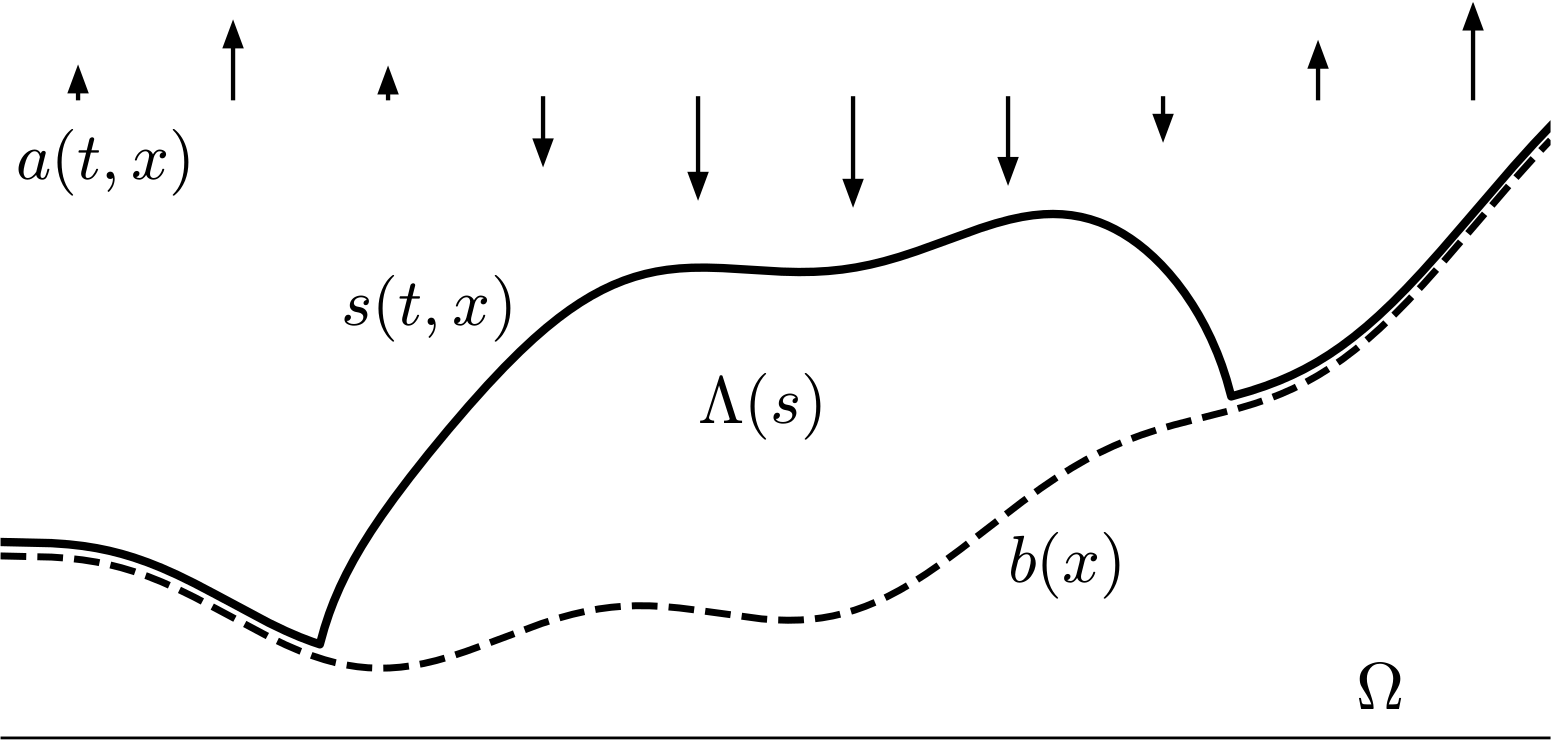
\includegraphics[width=0.65\textwidth]{genfigs/stokesdomain.pdf}
\caption{Notation for the glacier geometry problem used in this paper.}
\label{fig:stokesdomain}
\end{figure}

Let $s(t,x)$ be the solution surface elevation.  This surface must be above the bed ($s\ge b$).  Where there is ice there is a solution ice velocity $\bu(t,x,z)$ defined on the three-dimensional domain
\begin{equation}
\Lambda(t) = \left\{(x,z)\,:\,b(x) < z < s(t,x)\right\} \subset \Omega \times \RR. \label{eq:icydomain}
\end{equation}
It is important to emphasize this aspect of glacier models: the domain on which the ice flow velocity (and pressure) is meaningful is determined by the solution surface elevation $s$.

Suppose we denote the surface value (trace) of the velocity solution by $\bu|_s$.  Let $\bn_s = \left<-\grad s,1\right>$ denote an upward surface normal vector.  In strong form, what holds on all of $\Omega$ is an infinite-dimensional nonlinear complementarity problem (NCP) \cite{FacchineiPang2003}:
\begin{subequations}
\label{eq:ncp}
\begin{align}
s - b &\ge 0 \\
\frac{\partial s}{\partial t} - \bu|_s \cdot \bn_s - a &\ge 0 \\
(s - b) \left(\frac{\partial s}{\partial t} - \bu|_s \cdot \bn_s - a\right) &= 0
\end{align}
\end{subequations}
This NCP statement, which will be reformulated as a variational inequality (VI) \cite{KinderlehrerStampacchia1980} below, assumes the extension of $\bu|_s$ by zero outside of the (solution) glaciated area.

Thus, at a given map-plane location and time, either no glacier is present ($s=b$) or the surface kinematical equation (SKE) holds:
\begin{equation}
\frac{\partial s}{\partial t} - \bu|_s \cdot \bn_s - a = 0.  \label{eq:ske}
\end{equation}
This equation states that the non-material surface of the ice moves vertically according to the velocity of the ice particles at the surface plus the accumulation or ablation of ice; it is a statement of mass conservation at a non-material surface \cite{Aschwandenetal2012}.

However, within the ice a glacier simulation will conserve mass, here according to incompressibility, and it will conserve momentum.  Recalling definition \eqref{eq:icydomain}, let $\Gamma_s(t) \subset \partial \Lambda(t)$ be the upper surface $z=s$ and
$\Gamma_b(t) \subset \partial \Lambda(t)$ be the base $z=b$.  We now assume that the base of the ice is not sliding: $\bu_b=0$.  The standard model for such a glacier assumes a non-Newtonian Stokes problem \cite{GreveBlatter2009}.  Let $p(t,x,z)$ denote the (solution) pressure and $D\bu=\frac{1}{2}(\grad \bu + \grad \bu^{\top})$ the strain rate tensor.  The formula
\begin{equation}
\nu(D\bu) = \frac{\Gamma}{2} |D\bu|^{\pp-2} \label{eq:glen}
\end{equation}
defines the ice viscosity according to Glen's power law \cite{GreveBlatter2009}, in which the exponent $\pp$ is approximately 4.  The coefficient $\Gamma>0$ is determined by the measured properties of ice, and the fact that we assume it to be constant is (essentially) equivalent to saying that all the ice is at the same temperature.  Let $\rhoi$ be the density of ice and $\bg$ the acceleration of gravity.  Then the Stokes problem writes
\begin{subequations}
\label{eq:stokes}
\begin{align}
- \nabla \cdot \left(2 \nu(D\bu)\, D\bu\right) + \nabla p - \rhoi \bg &= \bzero && \text{within $\Lambda(t) \subset \RR^3$} \\
\nabla \cdot \bu &= 0 && \text{within $\Lambda(t) \subset \RR^3$} \\
\left(2 \nu(D\bu) D\bu - pI\right) \bn_s &= \bzero && \text{on $\Gamma_s(t)$} \\
\bu  &= 0 && \text{on $\Gamma_b(t)$}
\end{align}
\end{subequations}

In summary at this point, we assert that a non-shallow, non-sliding, and isothermal glacier simulation determines the evolution of the primary state variables $s(t,x)$, $\bu(t,x,z)$, and $p(t,x,z)$, from initial values of $s(0,x)$.  Because the flow is very viscous \cite{Acheson1990}, the Stokes problem \eqref{eq:stokes} determines $\bu(t,x,z)$ and $p(t,x,z)$ at each time, given $\Lambda(t)$.\footnote{The Stokes model acts as an instantaneous ``algebraic'' constraint on the evolution.  The coupled system \eqref{eq:ncp}, \eqref{eq:stokes} is both an infinite-dimensional differential algebraic equation (DAE) system and an infinite-dimensional NCP.}  The surface elevation $s$ is defined on $[0,T]\times \Omega$, but it is subject to the inequality constraint $s\ge b$.

In other words, a glacier simulation is an NCP \eqref{eq:ncp}, for a free-surface flow in a signed climate that can add or remove ice, coupled to a Stokes problem \eqref{eq:stokes} within the evolving, three-dimensional icy domain $\Lambda(t)$.  Such a simulation is generally formulated using a finite element (FE) method for the Stokes sub-problem.  To the author's knowledge all existing non-shallow models use a explicit time-stepping scheme to evolve the surface \cite[for example]{Jouvetetal2008}, with the one exception of the work \cite{WirbelJarosch2020}.  


\section{Implicit time-stepping variational inequality models} \label{sec:models}

Now we describe implicit time steps of the model in the Introduction.  Each step problem has a variational inequality (VI) weak formulation \cite{Evans2010,KinderlehrerStampacchia1980}.

In this VI we must choose whether to parameterize geometry as the glacier's surface elevation or its thickness.  While essentially equivalent at the level of the continuum problem, the surface elevation and thickness formulations have different character when FE approximations are applied and the later abstract estimate of section \ref{sec:abstractestimate} is considered.  In fact we start by formulating using surface elevation, and then state the version for thickness after that.  Surface elevation is preferred because of the effect illustrated in Figure \ref{fig:giscross}, that in observations of real land-based glaciers the surface elevation $s(t,x)$ is almost always smoother as a function of $x$ than the thickness $H(t,x) = s(t,x)-b(x)$.  As the Figure shows, the thickness ``inherits'' the lower regularity of the eroded and faulted bedrock elevation, while on the other hand the surface elevation is smoothed by flow.

\begin{figure}[ht]
\centering
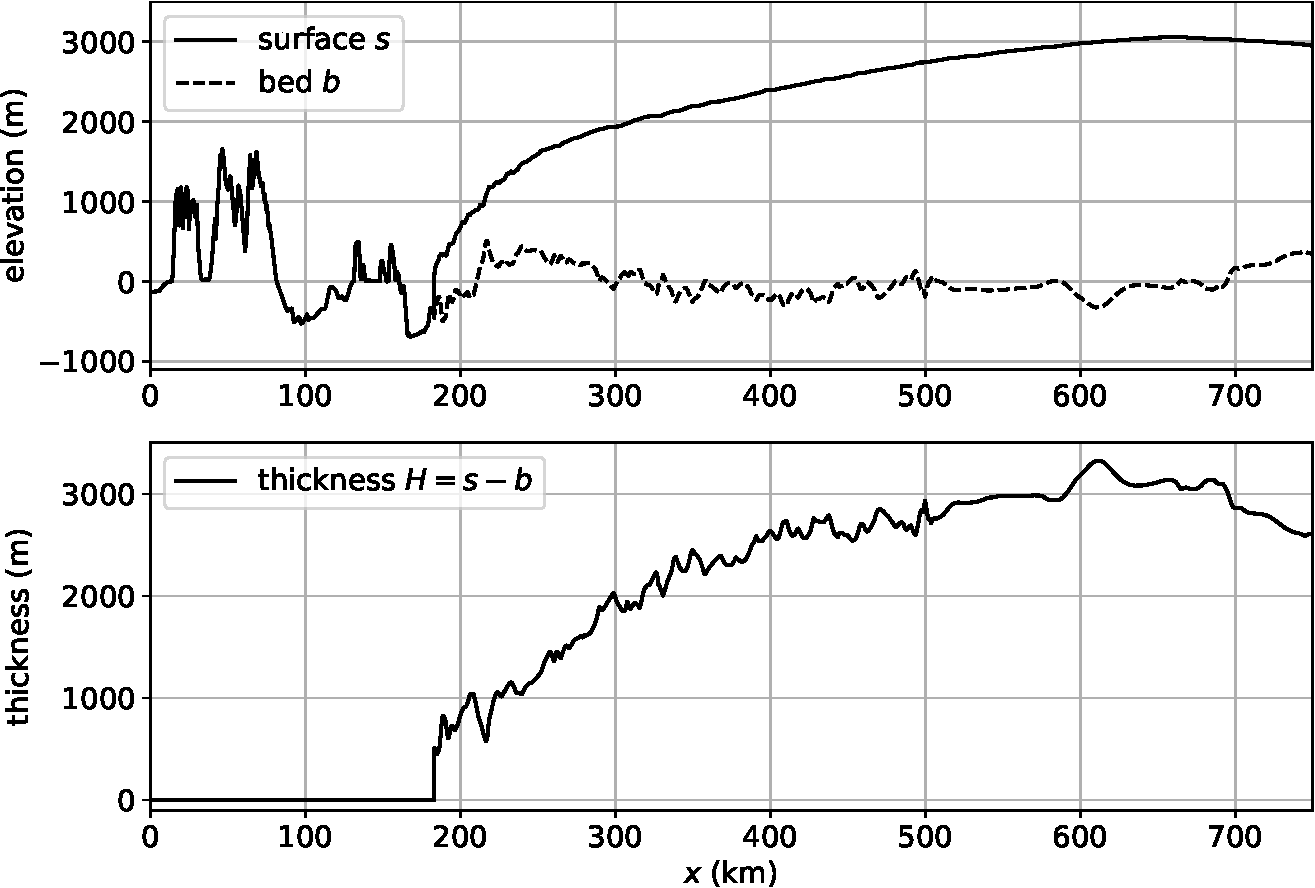
\includegraphics[width=0.85\textwidth]{genfigs/giscross.pdf}
\caption{A cross-section of the Greenland ice sheet at $70^\circ$N latitude (\cite{Morlighemetal2017} and A.~Aschwanden, personal communication; inset).  While the ice surface $s$ is relatively smooth because of ice flow (top), the bedrock elevation $b$ is much rougher.  The corresponding ice thickness $H = s-b$ (bottom), though it is a valid description of glacier geometry, inherits the low regularity of $b$.}
\label{fig:giscross}
\end{figure}

As in the Introduction, let $\Omega \subset \RR^2$ be a fixed region of land, suppose $b \in C^1(\Omega)$ is the time-independent bedrock elevation on $\Omega$, and, for $T>0$, let $a(t,x) \in C([0,T] \times \Omega)$ be the given surface mass balance (SMB) function.  Where $a(t,x)>0$ there is more snow in a year than can melt (accumulation), while if $a(t,x)<0$ the opposite is true (ablation).  Note that $a(t,x)$ is assumed to be defined everywhere in $\Omega$, regardless of whether a glacier is present or not, though necessarily $a(t,x) \le 0$ where there is no glacier.  At such an ablative location the value of $a(t,x)$ can be modeled using knowledge of precipitation plus an energy balance \cite{GreveBlatter2009}.  For example, one may hypothesize an ice or snow surface over an arbitrary depth of ice, then compute the total runoff from the available energy for melt, and then balance this against snow accumulation, if any.  In any case, $a(t,x)$ at an unglaciated location represents the SMB which a glacier would experience if it were present at that time and place.

Recall the surface kinematical equation (SKE) \eqref{eq:ske}, and the nonlinear complementarity problem (NCP) \eqref{eq:ncp} in which it appears.  Let $\{t_n\}$ be an increasing sequence of times, and, by abuse of notation, write $s(x) = s^n(x)\approx s(t_n,x)$ as the solution surface elevation at time $t_n$.  Using a backward Euler implicit step \cite{AscherPetzold1998}, the SKE is approximated by
\begin{equation}
\frac{s - s^{n-1}}{\Delta t} - \bu|_s \cdot \bn_s - a^n = 0. \label{eq:be:ske}
\end{equation}
where $\Delta t = t_n-t_{n-1}$ and $s^{n-1}(x) \approx s(t_{n-1},x)$.  For the SMB term $a^n$, assume that a temporal average has been computed.  Equivalently, let
\begin{equation}
\ell^n(x) = s^{n-1}(x) + \int_{t_{n-1}}^{t_n} a(t,x)\,dt; \label{eq:be:source}
\end{equation}
note $\ell^n=s^{n-1}+\Delta t\,a^n$.  The computable function $\ell^n$, which would be the updated surface elevation in the absence of flow, is a source term in what follows.  The implicit step solution $s$ will not, however, solve SKE \eqref{eq:be:ske} in all of $\Omega$.  Instead, similar to \eqref{eq:ncp}, an NCP holds:
\begin{subequations}
\label{eq:be:ncp}
\begin{align}
s - b &\ge 0 \label{eq:be:ncp:constraint} \\
s - \Delta t\,\bu|_s \cdot \bn_s - \ell^n &\ge 0 \\
(s - b) \left(s - \Delta t\,\bu|_s \cdot \bn_s - \ell^n\right) &= 0
\end{align}
\end{subequations}

The strong form NCP \eqref{eq:be:ncp} has a weak form VI which is suited to finite element (FE) approximation.  To state it we must hypothesize that surface elevations are in a Banach space $\cV$ of real-valued functions on $\Omega$.  (The precise space is unknown, but we will say more about it later in this Section.)  The admissible surface elevations are those which are above the bed, which defines a convex and closed subset:
\begin{equation}
\cK = \left\{r \in\cV\,:\,r \ge b\right\} \subset \cV.  \label{eq:be:admissible}
\end{equation}

To derive the VI form suppose $s$ is continuous and otherwise sufficiently regular so as to solve NCP \eqref{eq:be:ncp}.  The following argument is from \cite{Bueler2021conservation}.  Let $I$ be a measurable subset of $\Omega$ on which constraint \eqref{eq:be:ncp:constraint} is inactive, so a glacier is present on $I$: $I \subset \{x\,:\,s(x)>b(x)\}$.    Then, because the SKE \eqref{eq:be:ske} holds on all of $I$, it follows by integration that
\begin{equation}
\int_I \left(s - \Delta t\,\bu|_s \cdot \bn_s - \ell^n\right)\,(r-s) = 0.
\end{equation}
for all $r\in\cK$.  On the other hand, suppose $A \subset \Omega$ is measurable and a subset of the active region, i.e.~$A$ is in the ice-free region: $A \subset \{x\,:\,s(x)=b(x)\}$.  Note that $r-s=r-b\ge 0$ on $A$ for $r\in\cK$.  In this case we observe that $\ell^n - b = s^{n-1} - b + \Delta t\,a^n\le 0$ on all of $A$ because otherwise, using the continuity of $b$, $s^{n-1}$, and $a^n$, a glacier would still be present, or would have appeared, somewhere in $A$.  (Thus $s(x)>b(x)$ somewhere in $A$, a contradiction.)  Using $\bu|_s=0$ on $A$, i.e.~extension by zero, integration then shows an inequality because $b-\ell^n \ge 0$ and $r-s\ge 0$ on $A$:
\begin{equation}
\int_A \left(s - \Delta t\,\bu|_s \cdot \bn_s - \ell^n\right)\,(r-s) = \int_A \left(b - \ell^n\right)\,(r-b) \ge 0.
\end{equation}

Since all parts of $\Omega$ are either covered by glacier (in $I$) or ice free (in $A$), the argument above justifies the following VI model for the implicit time step solution surface elevation $s \in \cK$:
\begin{equation}
\int_\Omega \left(s - \Delta t\,\bu|_s \cdot \bn_s\right)\,(r-s) \ge \int_\Omega \ell^n \,(r-s) \quad \text{for all } r \in \cK. \label{eq:be:viearly}
\end{equation}
	
FIXME however we need to solve Stokes equations on $\Lambda(t)$ to get $\bu|_s$; here is weak form for that
\begin{equation}
XX \text{(see \cite{JouvetRappaz2011}, \cite{IsaacStadlerGhattas2015})} \label{eq:be:stokes}
\end{equation}
this is well posed \cite{JouvetRappaz2011}

FIXME now let
\begin{equation}
F(s) = s - \Delta t\,\Phi(s) \cdot \bn_s  \label{eq:be:Fdefine}
\end{equation}
and
\begin{equation}
\Phi(s) = \left(\text{trace of the solution $\bu$ of \eqref{eq:be:stokes} along upper surface $\Gamma_s$}\right)  \label{eq:be:Phidefine}
\end{equation}

FIXME restate VI: seek $s = s^n \in \cK$ so that 
\begin{equation}
\int_\Omega F(s)\,(r-s) \ge \int_\Omega \ell^n \,(r-s) \quad \text{for all } r \in \cK. \label{eq:be:vi}
\end{equation}

FIXME conjecture well-posedness of \eqref{eq:be:vi} for sufficiently short $\Delta t$

FIXME VI for mass continuity with $H$: fluid layer thickness equation, also called mass continuity or Saint Venant equation \cite{JouvetBueler2012}, $\cK = \{H\ge 0\}$, $\cK_h \subset \cK$, apparently $\eta = H^{2p/(p-1)} \in W^{1,p}(\Omega)$, for e.g.~$p=4$, because of existence in SIA case \cite{JouvetBueler2012}

FIXME SIA model has better-known properties \cite{JouvetBueler2012,PiersantiTemam2023}. however, regularity arising from analyzing SIA is not to be trusted because non-shallow (Stokes) dynamics is not diffusive for short wavelength surface/thickness perturbations \cite{Pattynetal2008}


\section{Abstract error estimate} \label{sec:abstractestimate}

We first consider an abstract variational inequality (VI) \cite{KinderlehrerStampacchia1980} problem as follows.  Let $\cV$ be a real reflexive Banach space with norm $\|\cdot\|$ and topological dual space $\cV'$.  Denote the dual pairing of $\phi \in \cV'$ and $v\in\cV$ by $\ip{\phi}{v} = \phi(v)$, and define the (Banach space) norm on $\cV'$ by $\|\phi\|_{\cV'} = \sup_{\|v\|=1} |\!\ip{\phi}{v}\!|$.

Let $\cK \subset \cV$ be a nonempty, closed, and convex subset, called the constraint set.  Elements of $\cK$ are said to be admissible.  For a continuous, but generally nonlinear, operator $f:\cK \to \cV'$, and a linear source $\ell\in \cV'$, the VI problem is to find $u\in \cK$ such that
\begin{equation}
\ip{f(u)}{v-u} \ge \ip{\ell}{v-u} \quad \text{for all } v\in \cK. \label{eq:vi}
\end{equation}
The best know example of \eqref{eq:vi} is the obstacle problem for the Laplacian operator; see e.g.~subsections 5.1 in \cite{Ciarlet2002} or 8.4.2 in \cite{Evans2010}.

\begin{definition} \label{def:monotonepcoercive}
An operator $f:\cK \to \cV'$ is said to be \emph{monotone} if
\begin{equation}
\ip{f(v)-f(w)}{v-w} \ge 0 \qquad \text{for all } v,w \in \cK \label{eq:monotone}
\end{equation}
and \emph{strictly monotone} if equality in \eqref{eq:monotone} implies $u=v$ \cite{KinderlehrerStampacchia1980}.  Let $p>1$.  The operator is \emph{$p$-coercive} \cite{Bueler2021conservation} if there exists $\alpha>0$ such that
\begin{equation}
\ip{f(v)-f(w)}{v-w} \ge \alpha \|v-w\|^p \qquad \text{for all } v,w \in \cK. \label{eq:pcoercive}
\end{equation}
\end{definition}

Clearly, if $f$ is $p$-coercive then it is monotone and strictly monotone, in which case any solution of \eqref{eq:vi} is unique.  Furthermore, it is well-known that if $f:\cK \to \cV'$ is also continuous on finite-dimensional subspaces then VI \eqref{eq:vi} has a solution \cite[Corollary III.1.8]{KinderlehrerStampacchia1980}.  Thus $p$-coercivity and appropriate continuity of $f$ show well-posedness for \eqref{eq:vi}.

% \cite{Peral1997} uniform continuity over bounded sets for p-Laplacian: Thm A.0.6

\begin{definition} \label{def:lipshitz}
For $\rho>0$ let $B_\rho = \{v\in \cV\,:\,\|v\|\le \rho\}$.  We say $f:\cK \to \cV'$ is \emph{Lipshitz on bounded sets of $\cK$} if for every $\rho>0$ there is $C(\rho)>0$ so that if $v,w \in B_\rho \cap \cK$ and $z\in\cV$ then $|\ip{f(v)-f(w)}{z}| \le C(\rho) \|v-w\| \|z\|$.  Equivalently:
\begin{equation}
\|f(v)-f(w)\|_{\cV'} \le C(\rho) \|v-w\| \quad \text{ for all } v,w \in B_\rho \cap \cK.  \label{eq:liponbounded}
\end{equation}
\end{definition}

Observe that in definitions \ref{def:monotonepcoercive} and \ref{def:lipshitz} we have only assumed $f$ is defined on $\cK$.

FIXME finite element space $\cV_h \subset \cV$, constraint set $\cK_h\subset \cV_h$, note generally $\cK_h \nsubseteq \cK$.  let $f_h:\cK_h\to\cV'$.  the FE VI problem is
\begin{equation}
\ip{f_h(u_h)}{v_h-u_h} \ge \ip{\ell}{v_h-u_h} \quad \text{for all } v_h\in \cK_h. \label{eq:fe:vi}
\end{equation}
we assume this problem is also well-posed FIXME FLESH OUT AND NOTE $f_h\ne f$ POSSIBLE

Now assume that $\cV$ continuously and densely embeds in a larger Banach space $\cB$:
\begin{equation}
\cV \hookrightarrow \cB, \quad \overline{\cV} = \cB
\end{equation}
Observe that $\cB' \subset \cV'$ is a Banach subspace.  Our main example will be where $\cV=W^{1,p}(\Omega)$ and $\cB=L^p(\Omega)$.  Compare the Hilbert-space case in \cite{Falk1974} and \cite[section 5.1]{Ciarlet2002}.

A key concept in what follows is that $f(u)-\ell$ is generally nonzero when $u$ solves \eqref{eq:vi}.  A nonlinear complementarity problem will hold, at least in sufficiently regular cases, as in \cite[Exercise 5.1.1]{Ciarlet2002}  and \cite[section 7]{BuelerFarrell2024}, for example.  Only for $u$ in the interior of $\cK$ should we expect equality $f(u)=\ell$.

In the following abstract error estimate, which significantly extends Theorem 5.1.1 in \cite{Ciarlet2002}, it is important to note that we now assume $f_h=f$ on a common extended domain of definition, namely $\hcK$ defined in \eqref{eq:convexhull}.  We also assume that $f(u)-\ell$ is a bounded linear functional on the larger space $\cB$.  However, we do not assume that $f$ is linear.

\begin{theorem} \label{thm:abstractestimate}
Let $1<p<\infty$ and let $q=p/(p-1)$ be the conjugate exponent.  Let
\begin{equation}
\hcK = \overline{\Hull{(\cK \cup \cK_h)}}  \label{eq:convexhull}
\end{equation}
be the closure (in $\cV$) of the convex hull of the union of the constraint sets $\cK$ and $\cK_h$.  Suppose that $f$ and $f_h$ can be extended to $\hcK$, and that they are the ``same'' map:
\begin{equation}
f:\hcK \to \cV', \, f_h:\hcK \cap \cV_h \to \cV', \, \text{ and } f=f_h \text{ on } \hcK \cap \cV_h.  \label{eq:commonextension}
\end{equation}
Assume $f$ is $p$-coercive over $\hcK$ with constant $\alpha>0$, and that it is Lipshitz on bounded sets of $\hcK$.  Suppose $u\in\cK$ solves \eqref{eq:vi} and $u_h\in\cK_h$ solves \eqref{eq:fe:vi}.  Assume that
\begin{equation}
\|f(u)-\ell\|_{\cB'} < \infty.  \label{eq:fellboundedB}
\end{equation}
Finally, let $R_h=\max\{\|u\|,\|u_h\|\}$.  Then there is a constant $c=c(\alpha,R_h)>0$ so that
\begin{align}
\|u-u_h\| &\le \Big(\inf_{v_h\in\cK_h} \left\{c \|u - v_h\|^q + \frac{2}{\alpha} \|f(u)-\ell\|_{\cB'} \|u-v_h\|_{\cB}\right\} \label{eq:abstractestimate} \\
   &\qquad + \inf_{v\in\cK} \frac{2}{\alpha} \|f(u)-\ell\|_{\cB'} \|u_h-v\|_{\cB}\Big)^{1/p} \notag
\end{align}
\end{theorem}

\begin{proof}  Let $v\in\cK$ and $v_h\in\cK_h$ be arbitrary.  Using \eqref{eq:commonextension}, rewrite VIs \eqref{eq:vi} and \eqref{eq:fe:vi}, as follows, no longer using $f_h$:
\begin{align*}
\ip{f(u)}{u}     &\le \ip{f(u)}{v} + \ell(u-v),  \\
\ip{f(u_h)}{u_h} &\le \ip{f(u_h)}{v_h} + \ell(u_h-v_h).
\end{align*}
It follows from these inequalities, plus $p$-coercivity over $\hcK$, that
\begin{align*}
\alpha \|u-u_h\|^p &\le \ip{f(u)-f(u_h)}{u-u_h} \\
  &= \ip{f(u)}{u} + \ip{f(u_h)}{u_h} - \ip{f(u)}{u_h} - \ip{f(u_h)}{u} \\
  &\le \ip{f(u)}{v} + \ell(u-v) + \ip{f(u_h)}{v_h} + \ell(u_h-v_h) \\
  &\qquad - \ip{f(u)}{u_h} - \ip{f(u_h)}{u} \\
  &= \ip{f(u)}{v-u_h} - \ell(v-u_h) \\
  &\qquad + \ip{f(u_h)}{v_h-u} - \ell(v_h-u) \\
  &= \ip{f(u)-\ell}{v-u_h} + \ip{f(u)-\ell}{v_h-u} \\
  &\qquad + \ip{f(u)-f(u_h)}{u-v_h}
\end{align*}
Since $u,u_h\in B_{R_h}$, by the Lipshitz assumption over $\hcK$ there is $C(R_h)>0$ so that $\|f(u)-f(u_h)\|_{\cV'} \le C(R_h) \|u-u_h\|$.  Also using the definition of $\|\cdot\|_{\cB'}$, from \eqref{eq:fellboundedB} it follows that
\begin{align*}
\alpha \|u-u_h\|^p &\le \|f(u)-\ell\|_{\cB'} \left(\|u_h-v\|_{\cB} + \|u-v_h\|_{\cB}\right) \\
  &\qquad + C(R_h) \|u-u_h\| \|u-v_h\|
\end{align*}
Now use Young's inequality with $\eps>0$ \cite[Appendix B.2]{Evans2010} on the final term:
\begin{align*}
\alpha \|u-u_h\|^p &\le \|f(u)-\ell\|_{\cB'} \left(\|u_h-v\|_{\cB} + \|u-v_h\|_{\cB}\right) \\
  &\qquad + C(R_h) \left(\eps\|u-u_h\|^p + \tilde C(\eps) \|u-v_h\|^q\right).
\end{align*}
(Here $\tilde C(\eps) = (\eps p)^{-q/p} q^{-1}$.)  Choose $\eps>0$ so that $C(R_h) \eps \le \alpha/2$, and subtract to find
\begin{align*}
\frac{\alpha}{2} \|u-u_h\|^p &\le \|f(u)-\ell\|_{\cB'} \left(\|u_h-v\|_{\cB} + \|u-v_h\|_{\cB}\right) \\
  &\qquad + C(R_h) \tilde C(\eps) \|u-v_h\|^q
\end{align*}
Take infimums to show \eqref{eq:abstractestimate}.
\end{proof}

As observed in \cite{Ciarlet2002}, the last quantity in \eqref{eq:abstractestimate}, involving $\|u_h-v\|$ for $v\in\cK$, is generally nonzero in obstacle problems where $\cK_h \nsubseteq \cK$.  This is relevant to glacier models tracking the surface elevation (as opposed to thickness).  In fact, consider obstacle problems where $\cK=\{v(x)\ge \psi(x)\}$, $\psi_h$ is an interpolant of $\psi$, and $\cK_h=\{v_h(x)\ge \psi_h(x)\}$.  Observe that, while $\psi_h(x_j)=\psi(x_j)$ for all interpolation nodes, generally $\psi_h(x) \ge \psi(x)$ does not hold for all $x\in\Omega$ even if $\psi$ is smooth.  That is, nodal admissiblity does not imply admissibility for surface elevations.

FIXME draw figure like Ciarlet Figure 5.1.3

On the other hand, it is worthwhile to consider situations with better data.  First, the complications related to the convex hull operation \eqref{eq:convexhull} disappear if the nonlinear operator $f=f_h$ is defined on all of $\cV$.  That is, if one replaces $\hcK$ with $\cV$ itself in Theorem \ref{thm:abstractestimate}, still assuming $f=f_h$ is $p$-coercive and Lipshitz on bounded sets of $\cV$, then \eqref{eq:abstractestimate} follows.

In fact, for linear operators defined on the entire vector space, Theorem \eqref{thm:abstractestimate} reduces to the abstract error estimate for variational inequalities given in \cite{Ciarlet2002} and \cite{Falk1974}.  Specifically, suppose $\ip{f(v)}{w}=a(v,w)$ is actually bilinear,\footnote{There is no need to assume $a(v,w)$ is symmetric.} $\cV$-elliptic, and continuous on a Hilbert space $\cV$.  Define $A:\cV\to\cV'$, a bounded linear operator, by $Av(w) = a(v,w)$. (Observe that continuity for $a(v,w)$ implies Lipshitz on bounded sets \eqref{eq:liponbounded} for $A$.  This is used in proving the Lax-Milgram lemma in \cite{Ciarlet2002}, for example.)  Suppose that $\cV\hookrightarrow \cH$ and $\overline{\cV} = \cH$ for some Hilbert space $\cH$, and that $\|Au-\ell\|_{\cH'} < \infty$ so that, up to isomorphism, $Au-\ell \in\cH$.  Then Theorem \ref{thm:abstractestimate} reduces to Theorem 5.1.1 of Ciarlet \cite{Ciarlet2002}, and to the result in Falk \cite{Falk1974}.

Next, the following corollary is relevant to glacier models solving for ice thickness (as opposed to surface elevation).  In this case $\cK = \{v\ge 0\}$ consists of all nonnegative functions and $\cK_h=\cK\cap\cV_h$, thus the last term in \eqref{eq:abstractestimate} is zero.

\begin{corollary}  \label{cor:abstractestimate:equalsets}
Suppose $\cK \supset \cK_h$.  Keeping the other assumptions of Theorem \ref{thm:abstractestimate}, it follows that
\begin{equation}
\|u-u_h\| \le \left(\inf_{v_h\in\cK_h} \left\{c \|u - v_h\|^q + \frac{2}{\alpha} \|f(u)-\ell\|_{\cB'} \|u-v_h\|_{\cB}\right\}\right)^{1/p}. \label{eq:abstractestimate:equalsets}
\end{equation}
\end{corollary}

Finally, if $f(u)=\ell$, for example if $u$ is in the interior of $\cK$, then $f(u)-\ell \in \cB'$ and the conclusion simplifies to, essentially, Cea's lemma \cite{Ciarlet2002}.  Note that we do not assume $\cK \supset \cK_h$ here, as in Corollary \ref{cor:abstractestimate:equalsets}.  The glacier situation here is that the entire domain $\Omega$ is covered in ice, with a positive minimum on the thicknesses.

\begin{corollary}  \label{cor:abstractestimate:interior}
Suppose $f(u)=\ell$.  Keeping the other assumptions of Theorem \ref{thm:abstractestimate}, it follows that there is $\tilde c>0$ so that
\begin{equation}
\|u-u_h\| \le \inf_{v_h\in\cK_h} \tilde c \|u - v_h\|^{q/p}. \label{eq:abstractestimate:interior}
\end{equation}
\end{corollary}




\section{Application of the estimate to glacier simulations} \label{sec:application}

FIXME apply Theorem \ref{thm:abstractestimate} and talk through what happens


\bibliographystyle{siamplain}
\bibliography{estimate}

\end{document}
